\documentclass[pdftex,12pt,a4paper]{report}

\usepackage{amsmath}
\usepackage{amsfonts}
\usepackage{amssymb}

\usepackage[ngerman]{babel}
\usepackage[utf8]{inputenc}


\usepackage[pdftex]{graphicx}
\usepackage{listings}

% new commands
\newcommand{\HRule}{\rule{\linewidth}{0.5mm}}


\author{Nik\v{s}a Ra\v{s}i\'{c};Martin Weinberg}
\title{Proposel Projekt}

\begin{document}
\title{Projektproposel:}
\date{09.01.13}
\author{Nik\v{s}a Ra\v{s}i\'{c} \& Martin Weinberg}

\begin{titlepage}
\begin{center}
% Upper part of the page
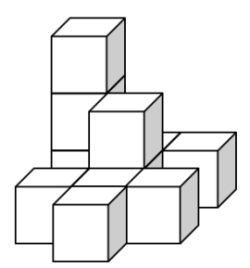
\includegraphics[width=0.4\textwidth]{./wuerfel}\\[1cm]    

\textsc{\LARGE Projektproposel}\\[1.5cm]

\textsc{\Large Creative Coding WS 12/13 }\\[0.5cm]


% Title
\HRule \\[0.4cm]
{ \huge \bfseries Emitting Cubes}\\[0.4cm]

\HRule \\[1.5cm]

% Author and supervisor
\begin{minipage}{0.4\textwidth}
\begin{flushleft} \large
\emph{Author:}\\
Nik\v{s}a Ra\v{s}i\'{c}  \&  \\ Martin Weinberg
\end{flushleft}
\end{minipage}
\begin{minipage}{0.4\textwidth}
\begin{flushright} \large
\emph{Supervisor:} \\ 
M. Sc.Alexander Neumann 
\end{flushright}
\end{minipage}

\vfill

% Bottom of the page
{\large \today}

\end{center}

\end{titlepage}

\tableofcontents
\newpage

\chapter{Emitting Cubes }
\section{Inspiration und Idee}
\section{Intention}
\section{Aufbau und Techniken}



\chapter{Konzepte mit Emitting Cubes}
\section{Die Partywürfel}
Die Würfel mit Effekten für den WOW-Effect

\section{Perspektivlosigkeit}
Die Würfel mti Kamerabildern aus verschiedeneen Perspektiven in die man sich reinfinden muss 

\end{document}






